\PassOptionsToPackage{table}{xcolor}

\documentclass[10pt]{beamer}
\usetheme[
%%% options passed to the outer theme
%    hidetitle,           % hide the (short) title in the sidebar
    hideauthor,          % hide the (short) author in the sidebar
%    hideinstitute,       % hide the (short) institute in the bottom of the sidebar
%    shownavsym,          % show the navigation symbols
%    width=2cm,           % width of the sidebar (default is 2 cm)
%    hideothersubsections,% hide all subsections but the subsections in the current section
%    hideallsubsections,  % hide all subsections
    left                % right of left position of sidebar (default is right)
  ]{Aalborg}
  
% If you want to change the colors of the various elements in the theme, edit and uncomment the following lines
% Change the bar and sidebar colors:
%\setbeamercolor{Aalborg}{fg=red!20,bg=red}
%\setbeamercolor{sidebar}{bg=red!20}
% Change the color of the structural elements:
%\setbeamercolor{structure}{fg=red}
% Change the frame title text color:
%\setbeamercolor{frametitle}{fg=blue}
% Change the normal text color background:
%\setbeamercolor{normal text}{bg=gray!10}
% ... and you can of course change a lot more - see the beamer user manual.
\definecolor{darkorange}{rgb}{.9,.3,0}
\definecolor{darkgray}{gray}{0.30}
\definecolor{lightgray}{gray}{0.90}
\setbeamercolor{alerted text}{fg=green}	%alert text

\usepackage[utf8]{inputenc}
\usepackage[spanish]{babel}
\usepackage[T1]{fontenc}
% Or whatever. Note that the encoding and the font should match. If T1
% does not look nice, try deleting the line with the fontenc.
\usepackage{iwona}
%\usepackage{helvet}

\usepackage{eurosym}
\usepackage{booktabs}

% colored hyperlinks
\newcommand{\chref}[2]{%
  \href{#1}{{\usebeamercolor[bg]{Aalborg}#2}}%
}

\title[\textbf{XRayDetector}]% optional, use only with long paper titles
{\textbf{XRayDetector}}

\subtitle{Detección automática de defectos en piezas metálicas\\mediante análisis de radiografías}  % could also be a conference name

\date{26 junio 2013}

\author[] % optional, use only with lots of authors
{
  Adrián González Duarte\\
  \href{mailto:agd0048@alu.ubu.es}{{\tt agd0048@alu.ubu.es}}\\
  Joaquín Bravo Panadero\\
  \href{mailto:jbp0023@alu.ubu.es}{{\tt jbp0023@alu.ubu.es}}
}

% - Give the names in the same order as they appear in the paper.
% - Use the \inst{?} command only if the authors have different
%   affiliation. See the beamer manual for an example

\institute[
  {
\includegraphics[scale=0.15]{AAUgraphics/escudo}}\\ %insert a company, department or university logo
  Ingeniería en Informática\\
  Universidad de Burgos
] % optional - is placed in the bottom of the sidebar on every slide
{% is placed on the bottom of the title page
  Ingeniería en Informática\\
  Universidad de Burgos
  
  %there must be an empty line above this line - otherwise some unwanted space is added between the university and the country (I do not know why;( )
}

% specify the logo in the top right/left of the slide
\pgfdeclareimage[height=1cm]{mainlogo}{AAUgraphics/logoXRayDetector.png} % placed in the upper left/right corner
\logo{\pgfuseimage{mainlogo}}

% specify a logo on the titlepage (you can specify additional logos an include them in 
% institute command below
\pgfdeclareimage[height=1.5cm]{titlepagelogo}{AAUgraphics/logoXRayDetector.png} % placed on the title page
\pgfdeclareimage[height=1.5cm]{titlepagelogo2}{AAUgraphics/escudo} % placed on the title page
\titlegraphic{% is placed on the bottom of the title page
  \pgfuseimage{titlepagelogo}
 \hspace{5cm}\pgfuseimage{titlepagelogo2}
}


%para poner las imágenes en cualquier posición
\newcommand{\putat}[3]{\begin{picture}(0,0)(0,0)\put(#1,#2){#3}\end{picture}}

%flechas
\usepackage{tikz}
\usetikzlibrary{shapes.arrows}


\tikzset{
    myarrow/.style={
        draw,
        fill=darkorange,
        single arrow,
        minimum height=3ex,
        single arrow head extend=1ex
    }
}

\newcommand{\arrowright}{%
\tikz [baseline=-0.5ex]{\node [myarrow] {};}
}

\makeatletter
\def\hlinewd#1{%
  \noalign{\ifnum0=`}\fi\hrule \@height #1 \futurelet
   \reserved@a\@xhline}
\makeatother


\begin{document}
% the titlepage
{\aauwavesbg
\begin{frame}[plain,noframenumbering] % the plain option removes the sidebar and header from the title page
  \titlepage
\end{frame}}
%%%%%%%%%%%%%%%%

% TOC
\begin{frame}{Índice}{}
\tableofcontents
\end{frame}
%%%%%%%%%%%%%%%%

\section{Introducción}
\begin{frame}{Introducción}{}
\begin{block}{Ensayos no destructivos (NDT)}

  \begin{itemize}
    \item Evitar destruir la pieza.
    \item En concreto, nos referimos a ensayos con \alert{radiografías}.
  \end{itemize}
  \putat{150}{-90}{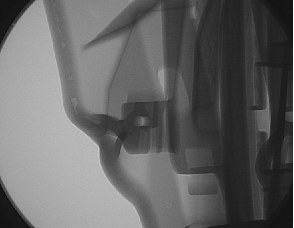
\includegraphics[scale=0.5]{AAUgraphics/radiografia.png}}  
  \pause
  \textbf{Ventajas}
  \begin{itemize}
    \item Método efectivo.
    \item Se revelan fallos internos.
  \end{itemize}
  \pause
  \textbf{Desventajas}
  \begin{itemize}
    \item Caro y lento.
    \item Personal cualificado.
    \item Contradicciones.
  \end{itemize}

\end{block}
\end{frame}

\section{Objetivos}
\begin{frame}{Objetivos}

 \begin{itemize}
    \item \alert{Rediseñar} la aplicación anterior.\newline 
    
	   
    
    \item Ampliar y mejorar la \alert{funcionalidad} de la aplicación previa:
    \begin{itemize}
      \item Mejorar la \alert{precisión}.
      \item Mejorar el \alert{rendimiento}.
      \item Añadir \alert{segmentación}.
      \item Añadir medidas de \alert{evaluación}.
    \end{itemize}
  \end{itemize}
  
  \putat{190}{80}{
\includegraphics[scale=0.1]{AAUgraphics/target.png}}

\end{frame}

\section{Conceptos teóricos}

\begin{frame}{Conceptos teóricos}{Esquema general visión por computador}

{\centering 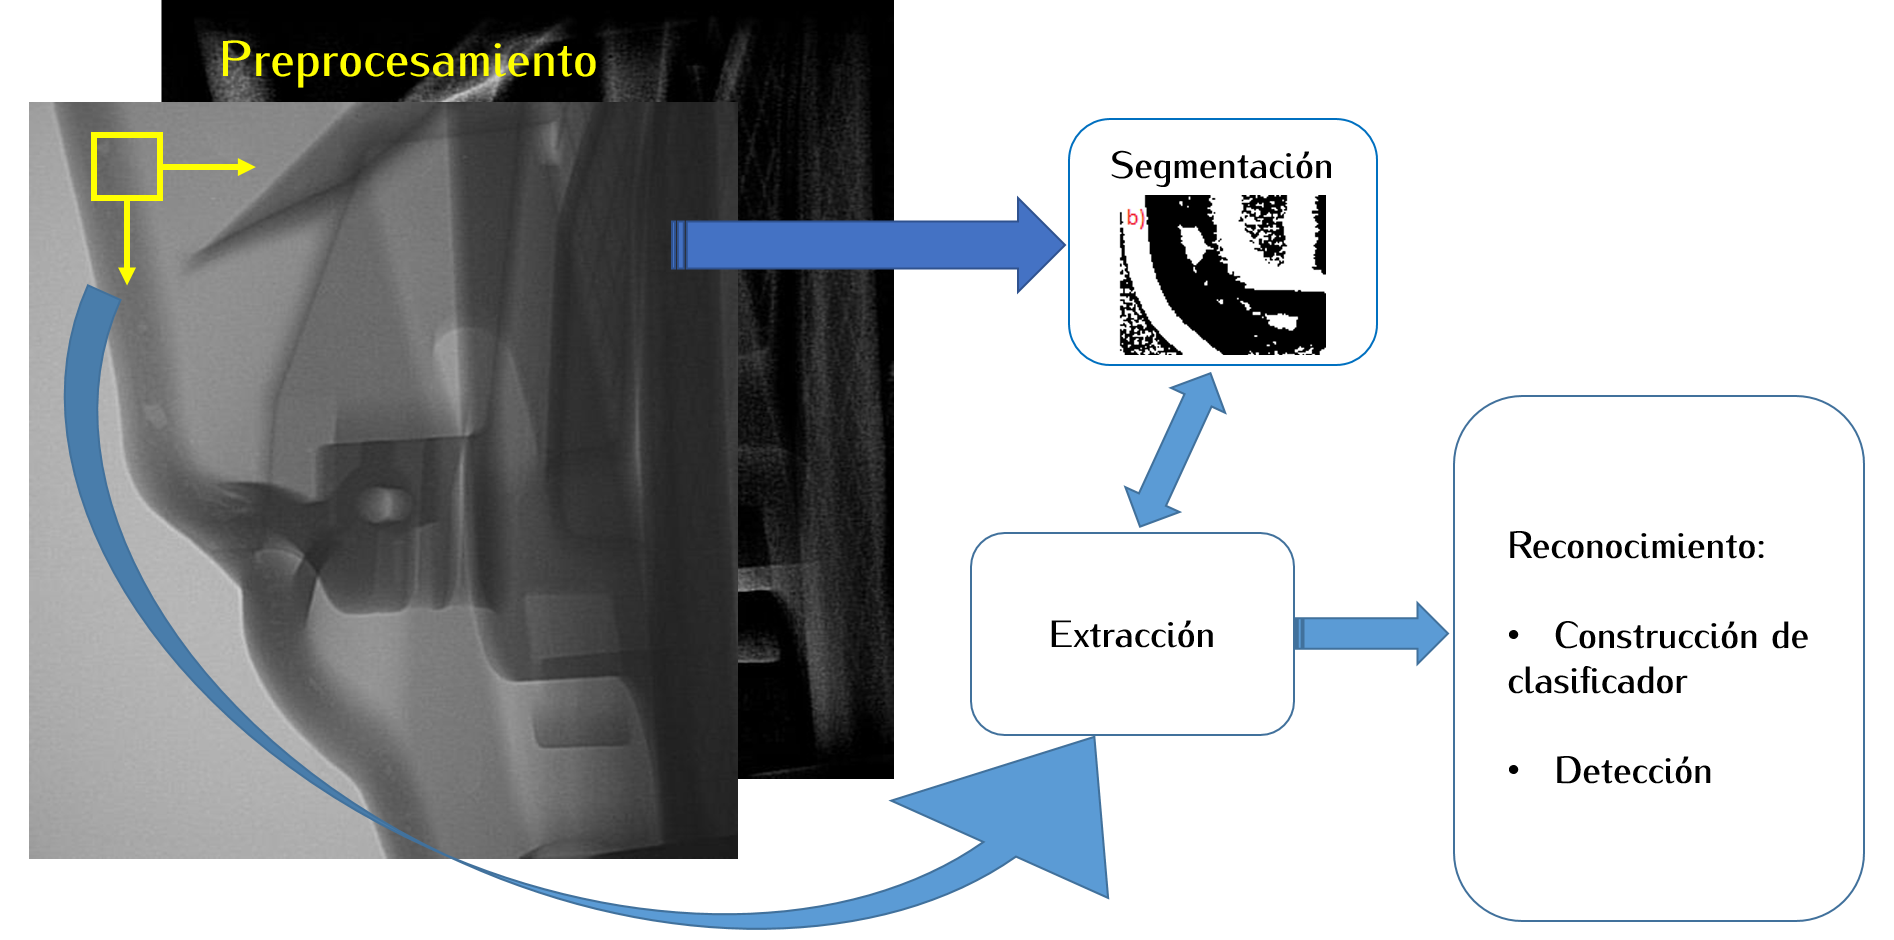
\includegraphics[scale=0.32]{AAUgraphics/proceso.png}\par}

\end{frame}


\subsection{Preprocesamiento}
\begin{frame}{Conceptos teóricos}{Preprocesamiento}
%Preprocesamiento

\begin{itemize}
\item Transformación de la información para facilitar la fase de análisis.
\end{itemize}

\pause

\begin{block}{Saliency Map}

\begin{itemize}
\item Prominencia visual de una imagen.
\item Identificar qué partes de la información deben ser seleccionadas para analizar.
\end{itemize}

{\centering 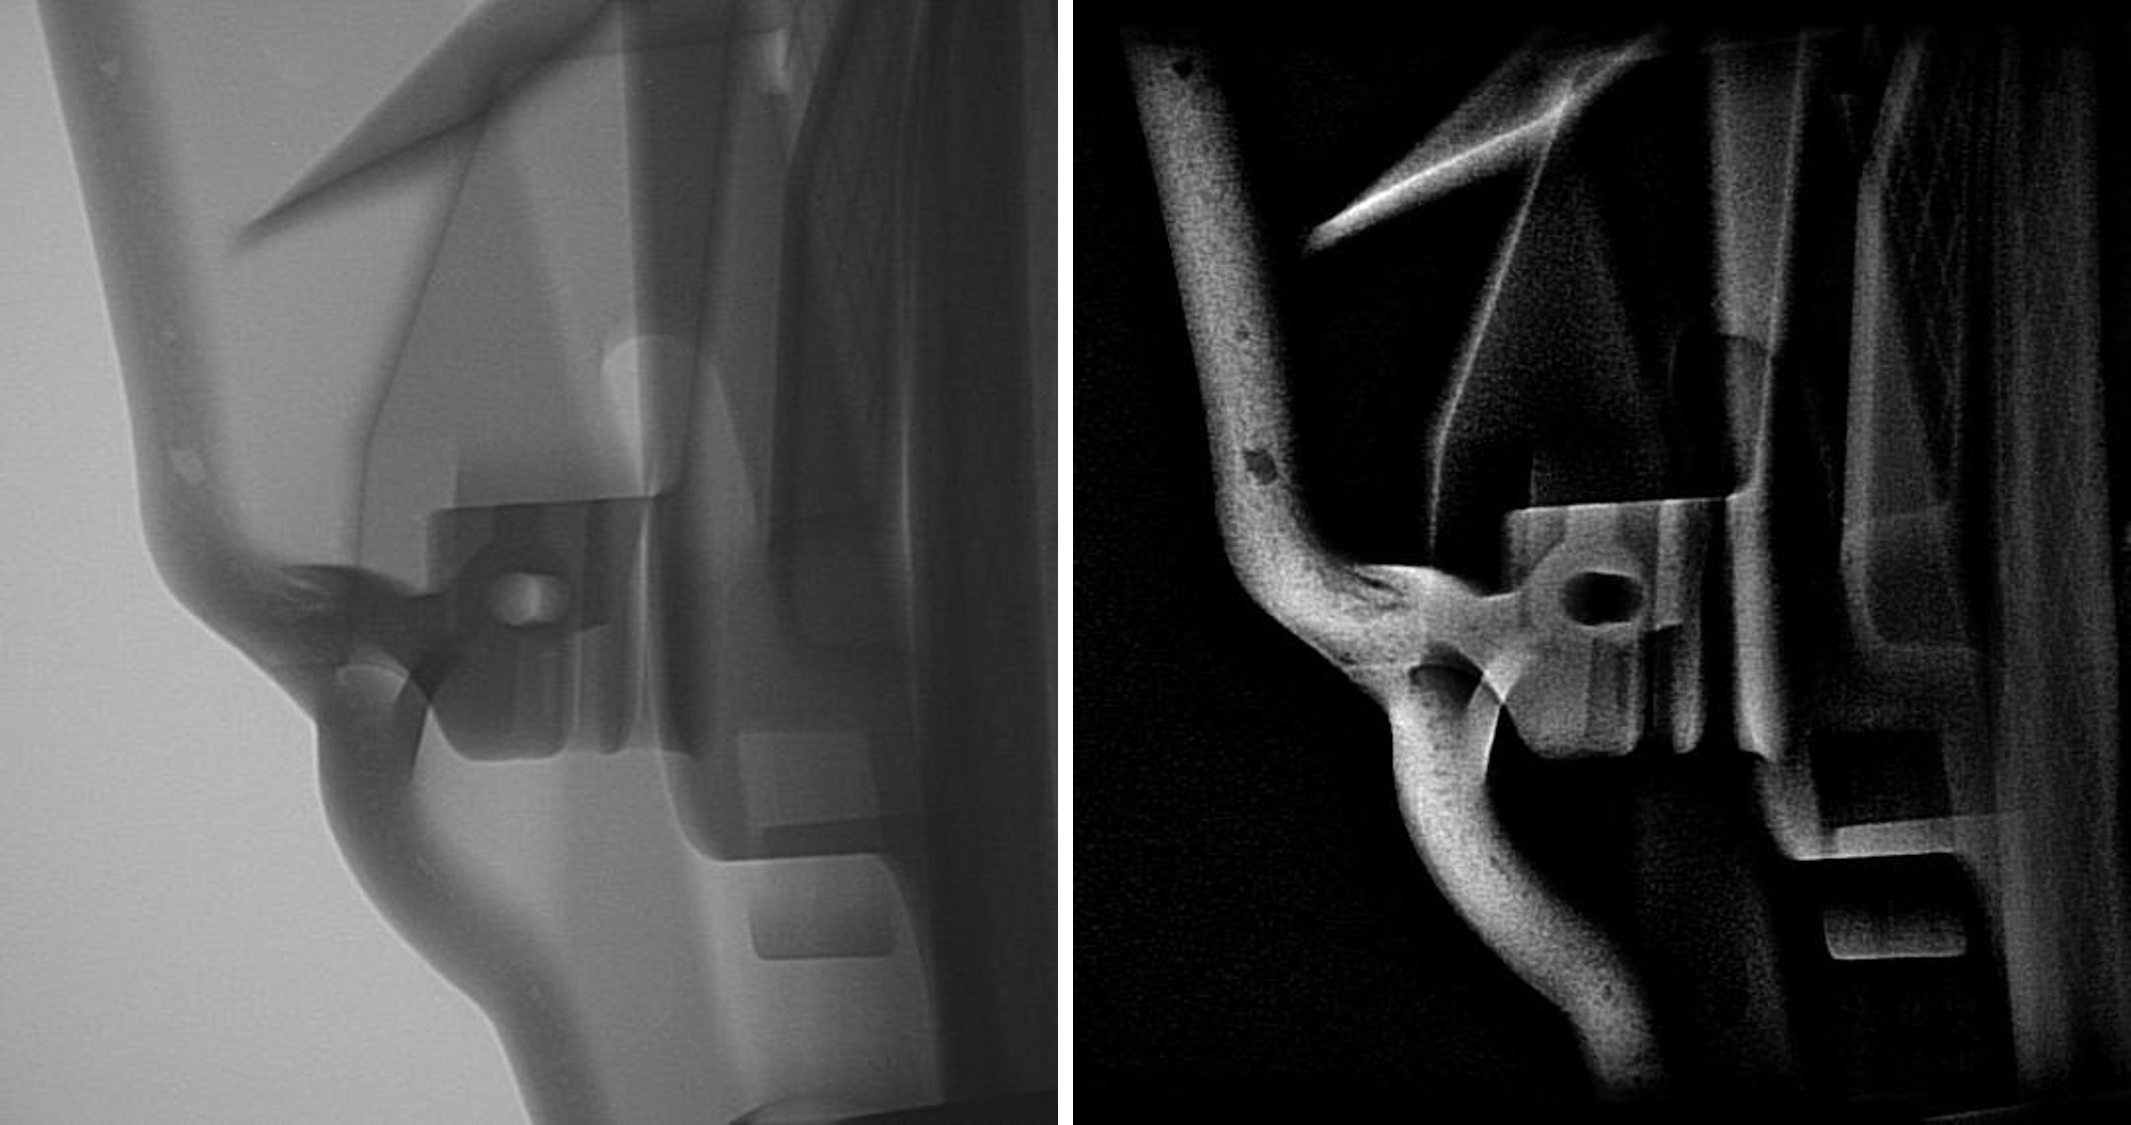
\includegraphics[scale=0.2]{AAUgraphics/saliency.png}\par}

\end{block}

\end{frame}

\subsection{Segmentación}
\begin{frame}{Conceptos teóricos}{Segmentación}

\begin{itemize}
\item Particionar una imagen en múltiples segmentos.
\item Localizar objetos y bordes.
\item Asignación de los píxeles a regiones (segmentos).\newline
\end{itemize}

\pause

\begin{block}{Thresholding}

\begin{itemize}
\item Umbral para binarizar la imagen.
\item \alert{Métodos locales:} umbral en cada píxel.

  \begin{itemize}
  \item \textbf{MidGrey}.
  \item \textbf{Mean}.
  \end{itemize}

\end{itemize}

\end{block}

\end{frame}

\subsection{Extracción}
\begin{frame}{Conceptos teóricos}{Extracción}

\begin{itemize}
\item Imagen lista para ser analizada.
\item Trabajamos directamente con los píxeles.
\end{itemize}

\pause

\begin{block}{Descriptores}

\begin{itemize}
\item \alert{Simples}
	\begin{itemize}
	\item Media.
	\item Desviación estándar.
	\item Primera y segunda derivadas.\newline
	\end{itemize}
\item \alert{De textura}
	\begin{itemize}
	\item Haralick.
	\item Local Binary Patterns (LBP).
	\end{itemize}
\end{itemize}

\end{block}

\end{frame}

%\begin{frame}{Conceptos teóricos}{Extracción - LBP}
%
%\begin{itemize}
%\item Gran capacidad de discriminación.
%\item Simplicidad de cálculo.
%\item Etiquetado de los píxeles comparando la intensidad de una región $3\times3$.
%\item \begin{tabular}{rc}
%Patrón & \arrowright  Histograma de patrones\\
%\end{tabular}
%\end{itemize}
%
%{\centering 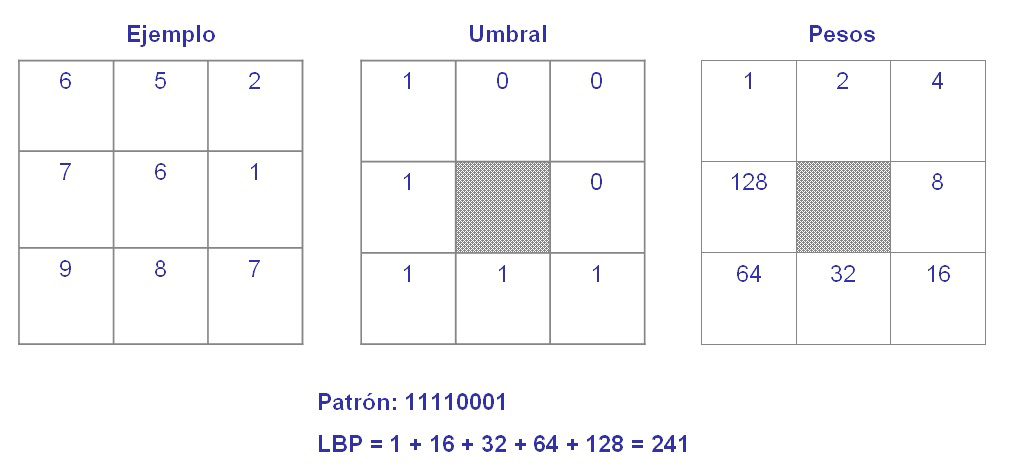
\includegraphics[scale=0.3]{AAUgraphics/lbp.png}\par}
%
%\end{frame}

\subsection{Reconocimiento de imágenes}
\begin{frame}{Conceptos teóricos}{Reconocimiento de imágenes}

\begin{itemize}
\item Entrenar un clasificador para predecir dónde estarán los defectos.
\item Aprender a partir de imágenes de ejemplo.
\end{itemize}

\pause

\begin{block}{Construcción del clasificador}
\begin{itemize}
\item Máscara de cada imagen (\alert{ground truth}):\newline

{\centering 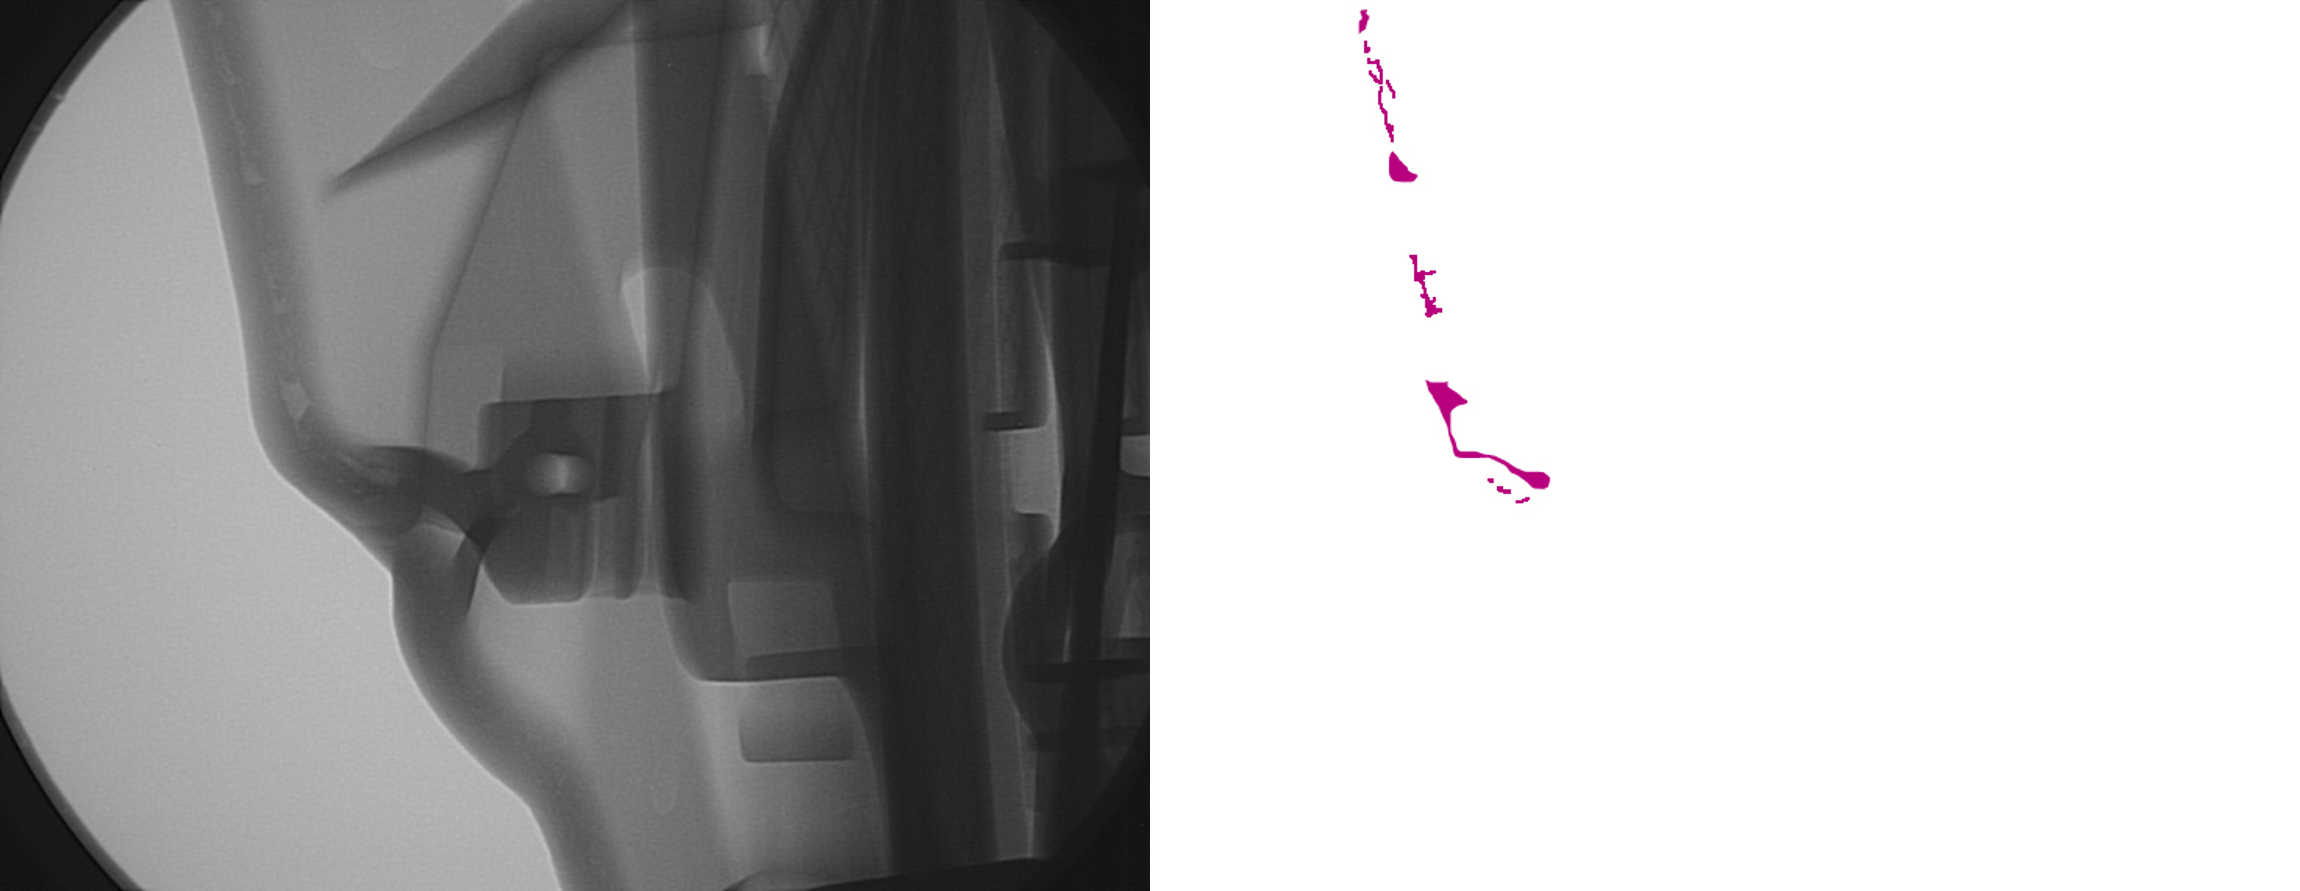
\includegraphics[scale=0.15]{AAUgraphics/mascara.png}\par}

\item Recorrer la imagen con una \alert{ventana} (aleatoria o deslizante).
\item Generación de vectores de características en ficheros \alert{ARFF}.

\end{itemize}
\end{block}

\end{frame}

\begin{frame}{Conceptos teóricos}{Reconocimiento de imágenes}

\begin{block}{Estrategias de etiquetado}
	\begin{itemize}
	\item Píxel central más región de vecinos.
	\item Porcentaje del total de la ventana.
	\end{itemize}
\end{block}

\pause

\begin{block}{Clasificador}
	\begin{itemize}
	\item \alert{Bagging} de \alert{REPTrees}.
	\end{itemize}
\end{block}

\pause

\begin{block}{Estrategias de detección}
	\begin{itemize}
	\item Normal.
	\item Normal más umbrales locales.
	\item Píxeles blancos en umbrales\\ locales.
	\end{itemize}
	
	\putat{160}{15}{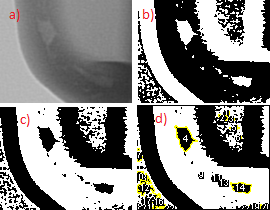
\includegraphics[scale=0.65]{AAUgraphics/segunda_opcion.png}}
\end{block}

\end{frame}

\section{Técnicas y herramientas}
\begin{frame}{Técnicas y herramientas}

{\centering 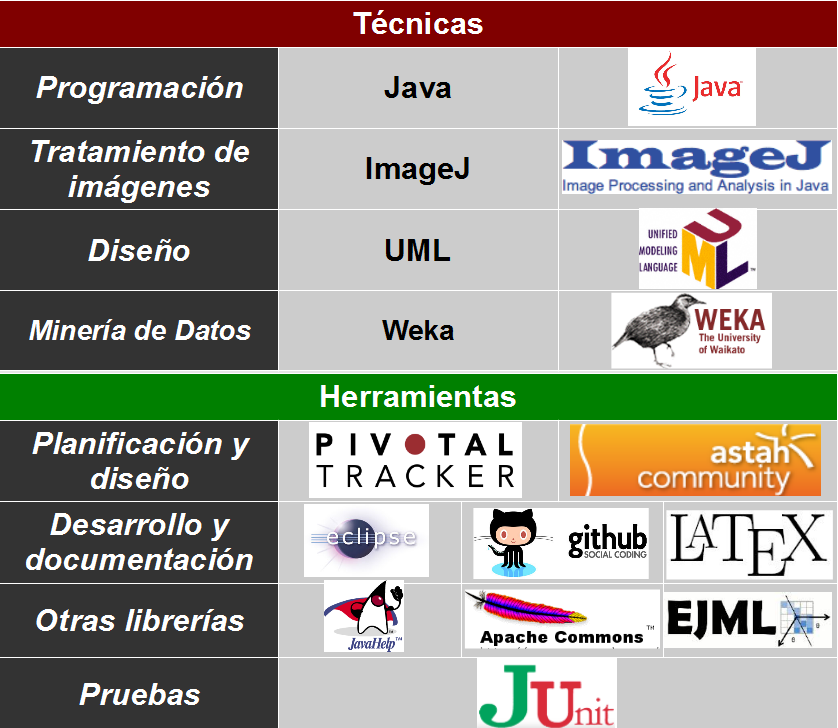
\includegraphics[scale=0.4]{AAUgraphics/tecnicas.png}\par}

%\centering
%\begin{tabular}{|>{\centering\arraybackslash} m{3cm} |>{\centering\arraybackslash} m{2.5cm} | >{\centering\arraybackslash}m{2.5cm} |}
%\hline
%\multicolumn{3}{|c|}{\cellcolor{red}\textcolor{white}{Técnicas}}\\
%\hline
%\cellcolor{darkgray}\textcolor{white}{Programación} & \cellcolor{lightgray}\textcolor{black}{Java} & 
\includegraphics[scale=0.25]{AAUgraphics/logojava.png}\\
%\hlinewd{1pt}
%\cellcolor{darkgray}\textcolor{white}{Imágenes} & \cellcolor{lightgray}\textcolor{black}{ImageJ} & 
\includegraphics[scale=0.3]{AAUgraphics/logoimagej.png}\\
%\hlinewd{1pt}
%\cellcolor{darkgray}\textcolor{white}{Diseño} & \cellcolor{lightgray}\textcolor{black}{UML} & 
\includegraphics[scale=0.15]{AAUgraphics/logouml.png}\\
%\hlinewd{1pt}
%\cellcolor{darkgray}\textcolor{white}{Minería de Datos} & \cellcolor{lightgray}\textcolor{black}{Weka} & 
\includegraphics[scale=0.2]{AAUgraphics/logoweka.png}\\
%\hline
%\end{tabular}
%
%\centering
%\begin{tabular}{|>{\centering\arraybackslash} m{3cm}|c|}
%\hline
%\multicolumn{2}{|c|}{\cellcolor{green}\textcolor{white}{Herramientas}}\\
%\hline
%\cellcolor{darkgray}\textcolor{white}{Planificación y diseño} & \begin{tabular}{>{\centering\arraybackslash} m{2.5cm} | >{\centering\arraybackslash}m{2.5cm} }
\includegraphics[scale=0.2]{AAUgraphics/logopivotal.png} & 
\includegraphics[scale=0.4]{AAUgraphics/logoastah.png}
%\end{tabular}\\
%\hlinewd{1pt}
%\cellcolor{darkgray}\textcolor{white}{Desarrollo y documentación} & \begin{tabular}{>{\centering\arraybackslash} m{1.67cm} | >{\centering\arraybackslash}m{1.67cm} | >{\centering\arraybackslash}m{1.66cm}}
%
%
\includegraphics[scale=0.5]{AAUgraphics/eclipselogo.png} & 
\includegraphics[scale=0.1]{AAUgraphics/gitlogo.png} & 
\includegraphics[scale=0.3]{AAUgraphics/latexlogo.png}
%\end{tabular}\\
%\hlinewd{1pt}
%
%\end{tabular}



\end{frame}


\section{Planificación}
\begin{frame}{Planificación}

\begin{itemize}
\item \alert{SCRUM}.
\item \textit{Product Backlog} con 42 \alert{historias de usuario}.
\item 11 iteraciones (\alert{sprints}).
\item Estimación basada en \alert{puntos}.
\end{itemize}

\begin{block}{Points breakdown chart}

\end{block}
{\centering 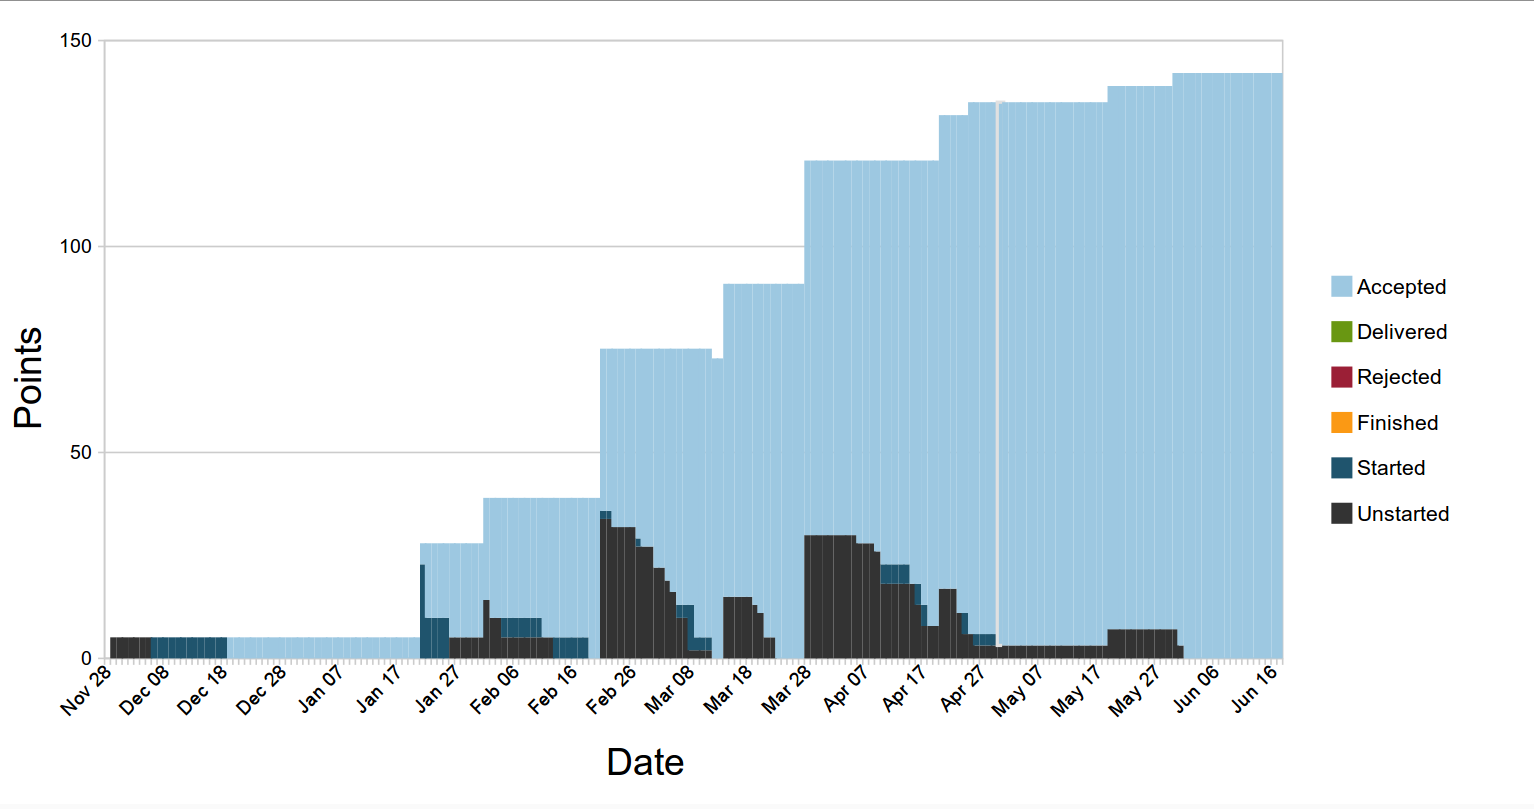
\includegraphics[scale=0.18]{AAUgraphics/planificacion.png}\par}
\end{frame}


\section{Viabilidad}
\begin{frame}{Viabilidad}{Viabilidad económica}

\begin{block}{Análisis de costes}
\vspace*{\baselineskip}
\centering
\begin{tabular}{| c | r |}
\hline
\cellcolor{beamer@headercolor}\textcolor{white}{Tipo} & \multicolumn{1}{ c }{\cellcolor{beamer@headercolor}\textcolor{white}{Coste}}\\
\hlinewd{1pt}
\cellcolor{lightgray}{Personal} & \cellcolor{lightgray}{19.065,60 \euro}\\
\hlinewd{1pt}
\cellcolor{lightgray}{Software} & \cellcolor{lightgray}{56,25 \euro}\\
\hlinewd{1pt}
\cellcolor{lightgray}{Hardware} & \cellcolor{lightgray}{333,33 \euro}\\
\hlinewd{1pt}
\cellcolor{lightgray}{Otros} & \cellcolor{lightgray}{3.016,00 \euro}\\
\hlinewd{1pt}
\cellcolor{gray}\textcolor{white}{\textit{Total}} & \cellcolor{gray}\textcolor{white}{\textit{22.471,18 \euro}}\\
\hline

\end{tabular}

\end{block}

\pause

\begin{block}{Análisis de beneficios}

\begin{itemize}
\item Destinado a uso industrial.
\item Coste licencia: 500 \euro.
\item \alert{Punto muerto}: 45 licencias.
\end{itemize}

\putat{180}{0}{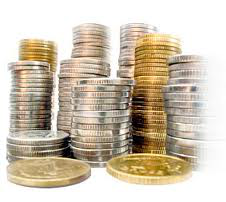
\includegraphics[scale=0.5]{AAUgraphics/money.png}}

\end{block}

\end{frame}


\begin{frame}{Viabilidad}{Viabilidad legal y técnica}

\begin{block}{Viabilidad legal}
\begin{itemize}
\item Licencia \alert{GNU}.
\item Heredada por librerías de terceros.
\end{itemize}

\putat{180}{0}{
\includegraphics[scale=0.1]{AAUgraphics/logognu.png}}

\end{block}

\pause

\begin{block}{Viabilidad técnica}
\begin{itemize}
\item El software utilizado en el proceso de desarrollo \alert{perdura} en el tiempo.
\item Software con utilidad \alert{real}.
\item \alert{Viable} desde el punto de vista técnico.
\end{itemize}
\end{block}

\end{frame}


\section{Aspectos relevantes}
\begin{frame}{Aspectos relevantes}
\begin{itemize}
\item \alert{Desconocimiento} de la base teórica.\newline


\item \alert{Complicaciones} para entender el proyecto anterior.\newline


\item Funcionalidad \alert{novedosa} e \alert{innovadora}.
\end{itemize}
\end{frame}


\section{Trabajos relacionados}
\begin{frame}{Trabajos relacionados}
\begin{itemize}
\item No existen aplicaciones comerciales.\newline


\item Gran cantidad de estudios y artículos.\newline


\item Proyecto europeo \textbf{MAGCAST}.
\end{itemize}
\end{frame}

\section{Demostración}
\begin{frame}{Demostración}
\begin{block}
{\centering 
\includegraphics[scale=0.4]{AAUgraphics/demo.png}\par}
\end{block}
\end{frame}


\section{Comparativa}
\begin{frame}{Comparativa}{Mejoras}
\begin{itemize}
\item Mejoras sobre el código fuente.
\item Mejoras sobre la estructura.
\item Mejoras en la precisión.
\item Mejoras en el rendimiento.
\item Mejoras sobre la interfaz.
\item Mejoras en la documentación y ayuda.
\item Mayor funcionalidad.
\end{itemize}

\putat{190}{50}{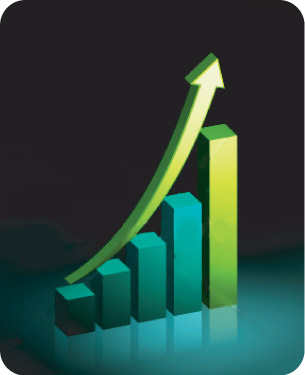
\includegraphics[scale=0.2]{AAUgraphics/mejora.jpg}}

\end{frame}

\begin{frame}{Comparativa}{Métricas}

\begin{block}
{\centering 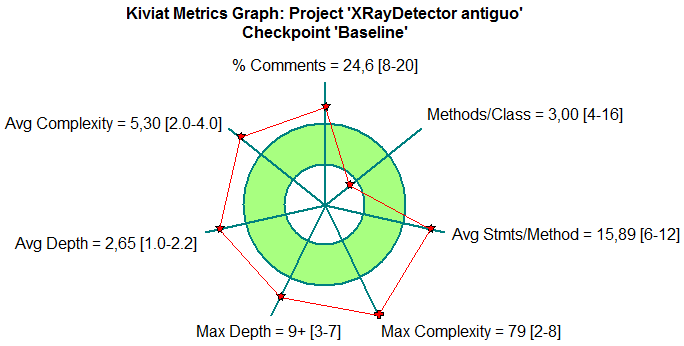
\includegraphics[scale=0.4]{AAUgraphics/kiviat2.png}\par}

{\centering 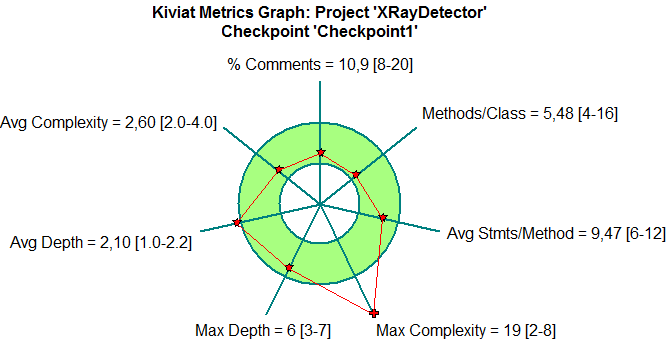
\includegraphics[scale=0.4]{AAUgraphics/kiviat1.png}\par}
\end{block}

\end{frame}


\section{Conclusiones y líneas futuras}
\begin{frame}{Conclusiones}
\begin{itemize}
\item Aprendizaje de nuevas técnicas y herramientas.\newline


\item Proyecto de carácter científico. Experimentación.\newline


\item Se han satisfecho todos los objetivos marcados.\newline


\item Experiencia enriquecedora y positiva.
\end{itemize}

\end{frame}

\begin{frame}{Líneas futuras}
\begin{itemize}
\item Clasificación de los defectos en tipos.\newline
\item Cálculo de nuevas características.\newline
\item Nuevas estrategias de detección.\newline
\item Uso de operadores morfológicos (dilatación y erosión).\newline
\item Ejecución en un supercomputador.\newline
\item Ampliación a otros campos.\newline
\item Arquitectura cliente-servidor.\newline
\end{itemize}

\putat{195}{125}{
\includegraphics[scale=0.7]{AAUgraphics/bombilla.png}}

\end{frame}

%\section*{Agradecimientos}


{\aauwavesbg%
\begin{frame}[plain,noframenumbering]{Agradecimientos}
  \begin{block}{Tutores}
  \begin{itemize}
    \item Dr. César I. García Osorio.
    \item José Francisco Díez Pastor.
  \end{itemize}
  \end{block}
  
  \begin{block}{Otros}
  \begin{itemize}
    \item Profesores de la carrera.
    \item Otros compañeros.
    \item Familiares y amigos.
  \end{itemize}
  \end{block}
\end{frame}}



{\aauwavesbg%
\begin{frame}[plain,noframenumbering]{Preguntas}
  \questionspage{{\centering 
\includegraphics[scale=0.2]{AAUgraphics/question.png}\par}}
\end{frame}}

{\aauwavesbg%
\begin{frame}[plain,noframenumbering]%
  \finalpage{Muchas gracias por su atención}
\end{frame}}



\end{document}
